\chapter{Análisis}

El proyecto surge  a raíz de la necesidad de SWAD de un editor integrado, que permita el formato de los textos. SWAD es una plataforma muy completa en lo que a gestión docente se refiere, pero si hay un punto débil en esta es la incapacidad de un usuario de dar formato al contenido que genera o lo que es incluso más importante, insertar fórmulas matemáticas. 

\section{Requisitos funcionales}

Los requisitos de nuestro editor son los siguientes:

\begin{itemize}
\item \textbf{Simplicidad} en su uso. El usuario deberá ser capaz de usar el editor sin una fase de entrenamiento previa, cometiendo como máximo un error por cada veinte minutos de uso. 

Dado que SWAD es una plataforma usada por muchos profesores y alumnos de muy diversas titulaciones el editor debe ser lo mas simple e intuitivo posible, evitando en la representación del contenido notación HTML, bbcode o similares. Estos editores son los que se conoce como editores WYSIWYG (What You See Is What You Get).

\item Fácil \textbf{integración} con SWAD. La integración del editor en la plataforma no requerirá más de tres líneas en el código de la plataforma. Nuestro editor debe ser lo mas independiente de SWAD posible, integrándose él mismo en el código de la página HTML. 

\item Soporte para \textbf{fórmulas} matemáticas. Nuestro editor permitirá insertar fórmulas matemáticas. Además, se contemplará la posibilidad de visualización de una página con múltiples fórmulas matemáticas sin que se produzca un deterioro excesivo del rendimiento (Tiempo de carga medio de 10 fórmulas inferior a 1 segundo).

\item Inserción de \textbf{símbolos}. Nuestro editor permitirá la inserción de símbolos tales como letras griegas y operadores matemáticos y algebraicos.

\item Posibilidad de ver y editar el \textbf{código HTML} generado, así como generar un código HTML de calidad, controlando etiquetas no cerradas y bloqueando etiquetas no permitidas para que el contenido global de la página no se vea afectado y evitar ataques XSS respectivamente.

\item \textbf{Formato simple de texto} y su estructura. Principalmente negrita, cursiva, subrayado, tachado y viñetas, subíndices, superíndices así como formato de cabeceras y cuerpo de texto y tipos de letra normal y mono-espaciada. 

\item El editor permitirá añadir \textbf{imágenes} y \textbf{enlaces}.

\item \textbf{Disponibilidad} del servicio. Por eso no debemos usar ninguna herramienta online, ya que no tenemos ninguna garantía de la continuidad de estos servicios. Por el mismo motivo usaremos tecnologías poco susceptibles de cambio, para reducir de esta manera las posibles labores de mantenimiento.

\item \textbf{Seguridad}. Permitir al usuario modificar directamente el HTML de la página conlleva un grave riesgo para la seguridad del sistema. Por ello, debemos filtrar el HTML generado con el fin de evitar las amenazas de inyección de código malicioso (XSS) en la plataforma.

\end{itemize}

\section{Visión global de la solución}
De lo anteriormente expuesto, podemos extraer que en el lado del cliente (Navegador Web) se dará formato al texto que introducimos, mientras que en el lado del servidor nos ocuparemos de generar las imágenes de las fórmulas y limpiar el código HTML generado.

Generando las imágenes de las fórmulas en el servidor nos aseguramos de que se cumple el requisito de tiempo impuesto a la carga de imágenes. Aunque puede producirse un pequeño deterioro en el rendimiento al cargar las imágenes, esto ocurrirá solo la primera vez ya que la caché del navegador hará que la carga las veces posteriores sea imperceptible. 

\section{Integración en la Plataforma}

En esta sección analizaremos las distintas partes de la plataforma SWAD en las que es necesario el uso del editor SWADE. Es importante un análisis de los lugares de la plataforma en los que se insertará el editor para que el diseño de la solución se adapte de la forma mas simple y elegante posible a cada caso.

Usaremos el editor SWADE para introducir la información de las distintas asignaturas. Dados de alta como profesores, en la pestaña Asignatura, debemos usar el editor en las secciones Introducción, Guía docente, Programa teoría, Programa prácticas,  Bibliografía, FAQ, Enlaces y en la pestaña Evaluación a la sección Sistema de Evaluación. En la figura ~\ref{fig:asig} podemos ver las distintas secciones donde vamos a integrar el editor.


\begin{figure}
        \centering
        \begin{subfigure}[b]{0.3\textwidth}
                
\includegraphics[width=\textwidth]{fig/inte_asig1}
                %\caption{A gull}
                \label{fig:inte_asig1}
        \end{subfigure}%
        ~ %add desired spacing between images, e. g. ~, \quad, \qquad etc.
          %(or a blank line to force the subfigure onto a new line)
        \begin{subfigure}[b]{0.3\textwidth}
                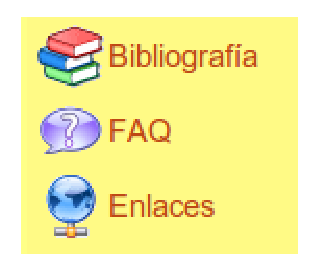
\includegraphics[width=\textwidth]{fig/inte_asig2}
                %\caption{A tiger}
                \label{fig:inte_asig2}
        \end{subfigure}
        ~ %add desired spacing between images, e. g. ~, \quad, \qquad etc.
          %(or a blank line to force the subfigure onto a new line)
        \begin{subfigure}[b]{0.3\textwidth}
                
\includegraphics[width=\textwidth]{fig/inte_eva}
                %\caption{A mouse}
                \label{fig:inte_eva}
        \end{subfigure}
        \caption{Secciones de info. asignaturas donde vamos a integrar SWADE }\label{fig:asig}
\end{figure}


En todas estas opciones, en el menú de edición, se nos preguntará el método por el que vamos a editar dicha sección, donde podremos seleccionar nuestro editor, tal como podemos ver en la figura ~\ref{fig:inte_sel}. 
  

\begin{figure}[h!]
  \centering
      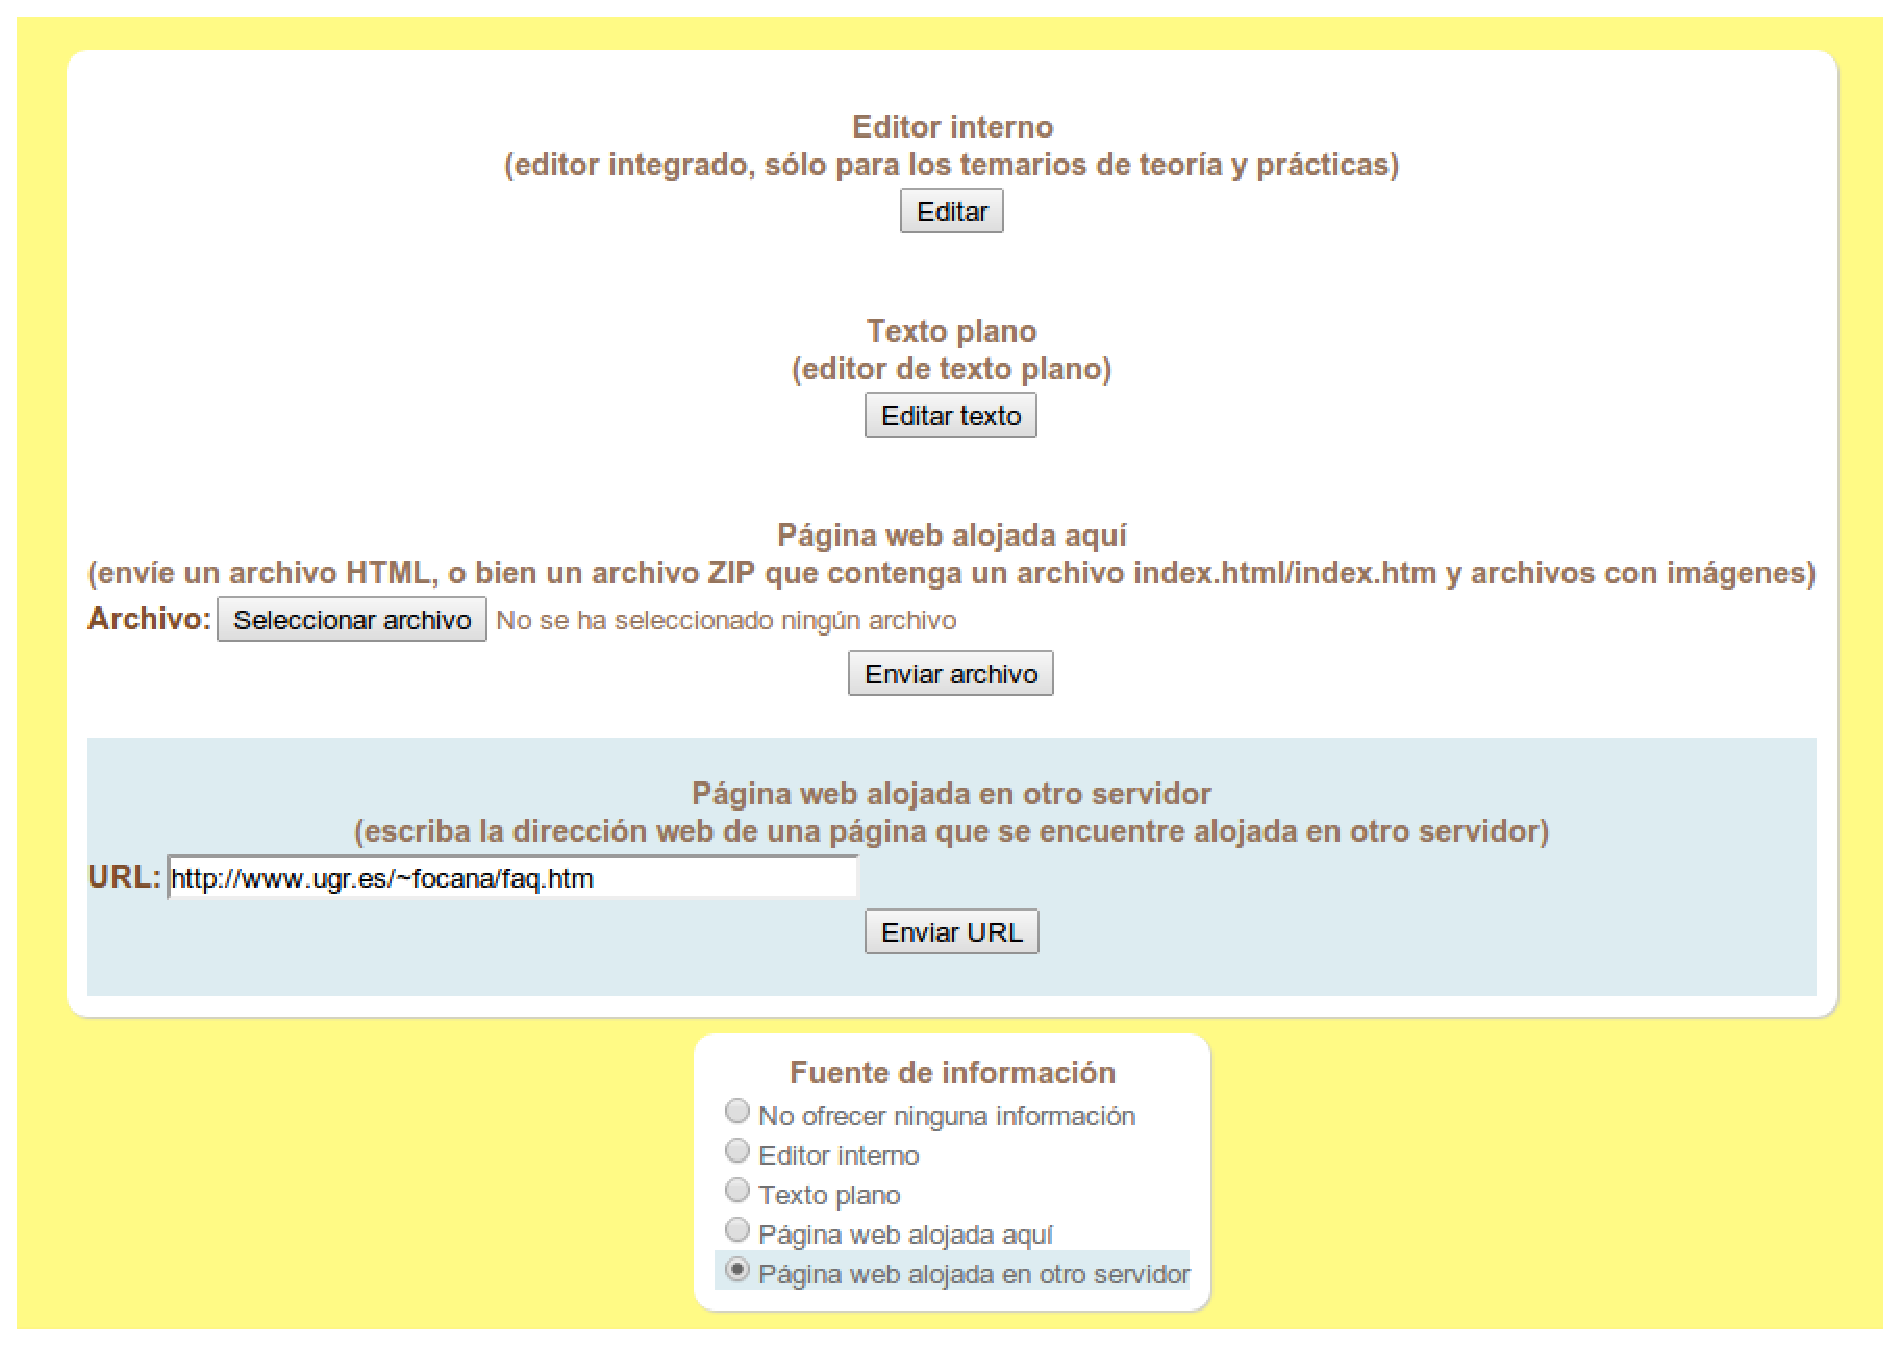
\includegraphics[width=7in]{fig/inte_sel}
  \caption{Menú de selección de método de edición.}
  \label{fig:inte_sel}

\end{figure}


También será necesario integrar SWADE en el campo descripción de Actividades y Encuestas de las pestañas Evaluación y Estadísticas respectivamente. En la figura ~\ref{fig:inte_acti} podemos ver el formulario de creación de una nueva actividad. El formulario de creación de una nueva encuesta es muy similar.

\begin{figure}[h!]
  \centering
      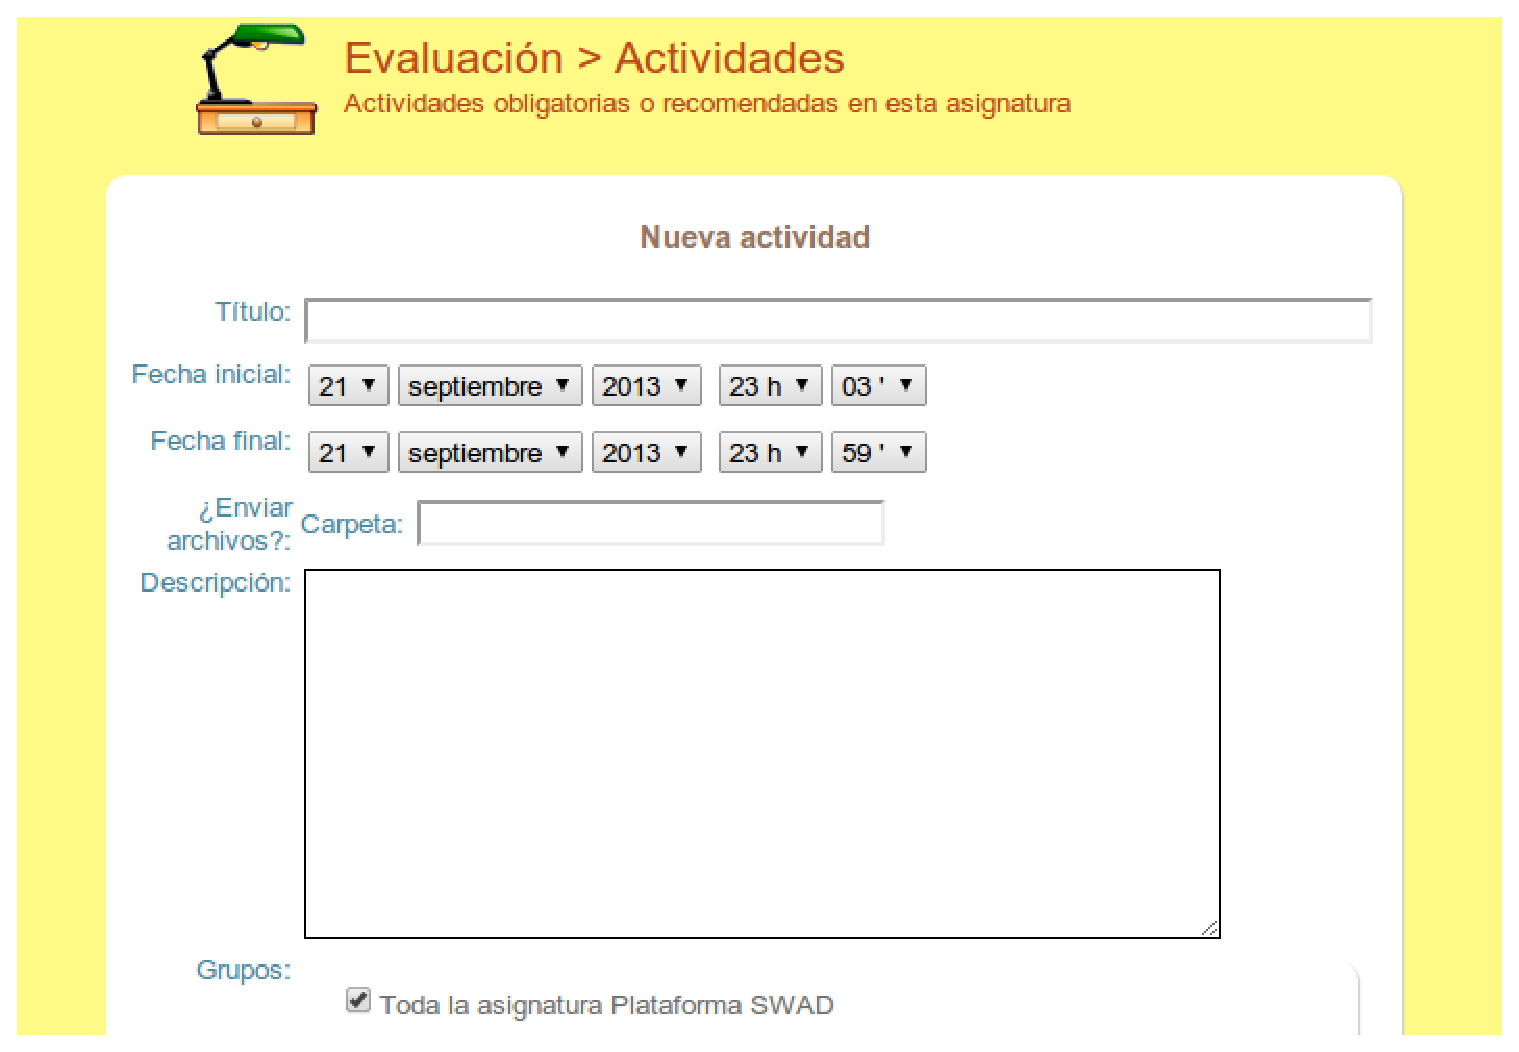
\includegraphics[width=4in]{fig/inte_acti}
  \caption{Creación de una nueva actividad.}
  \label{fig:inte_acti}

\end{figure}


Debemos contemplar también la posibilidad de creación de múltiples editores en un mismo documento HTML ya que, en la sección de Test de la pestaña Evaluación, debemos insertar un total de veintidós editores cada vez que creamos una nueva pregunta. Serían dos por cada posible respuesta, haciendo un total de veinte, más dos por el enunciado y la realimentación de este. En las figuras ~\ref{fig:inte_test1} e ~\ref{fig:inte_test2} podemos ver el formulario de creación de una nueva pregunta de test.

\begin{figure}[h!]
  \centering
      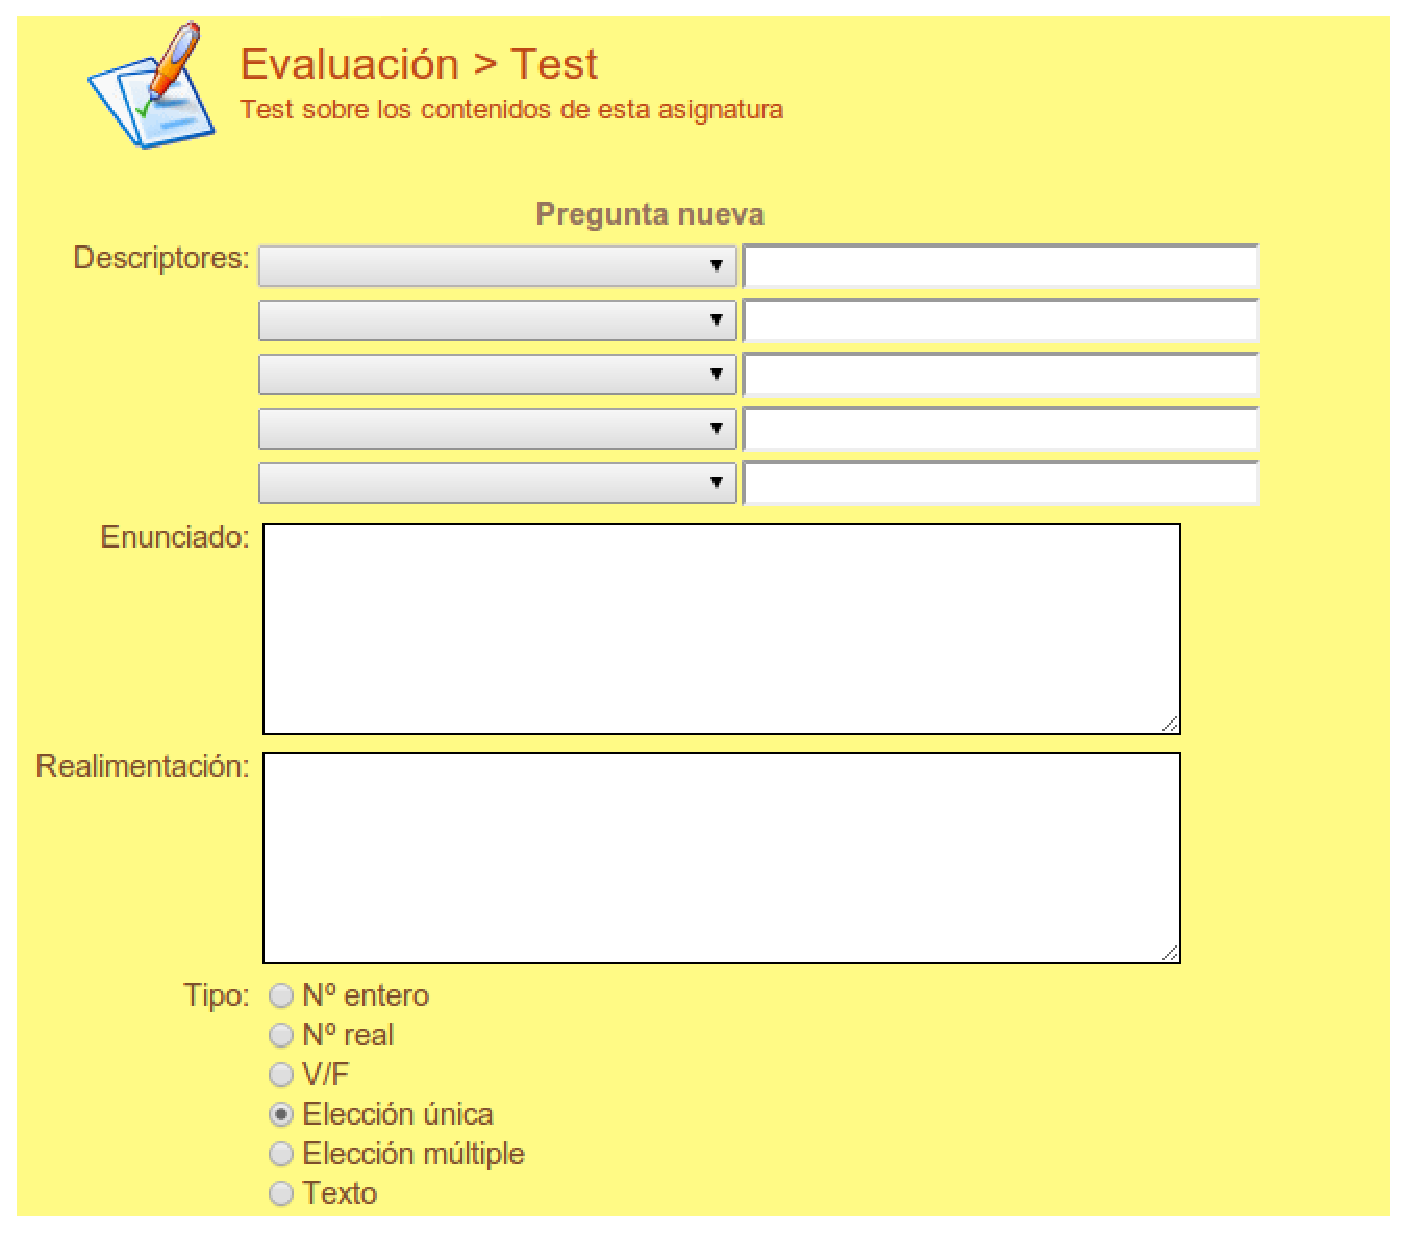
\includegraphics[width=4in]{fig/inte_test1}
  \caption{Creación de un nuevo test. Enunciado.}
  \label{fig:inte_test1}

\end{figure}

\begin{figure}[h!]
  \centering
      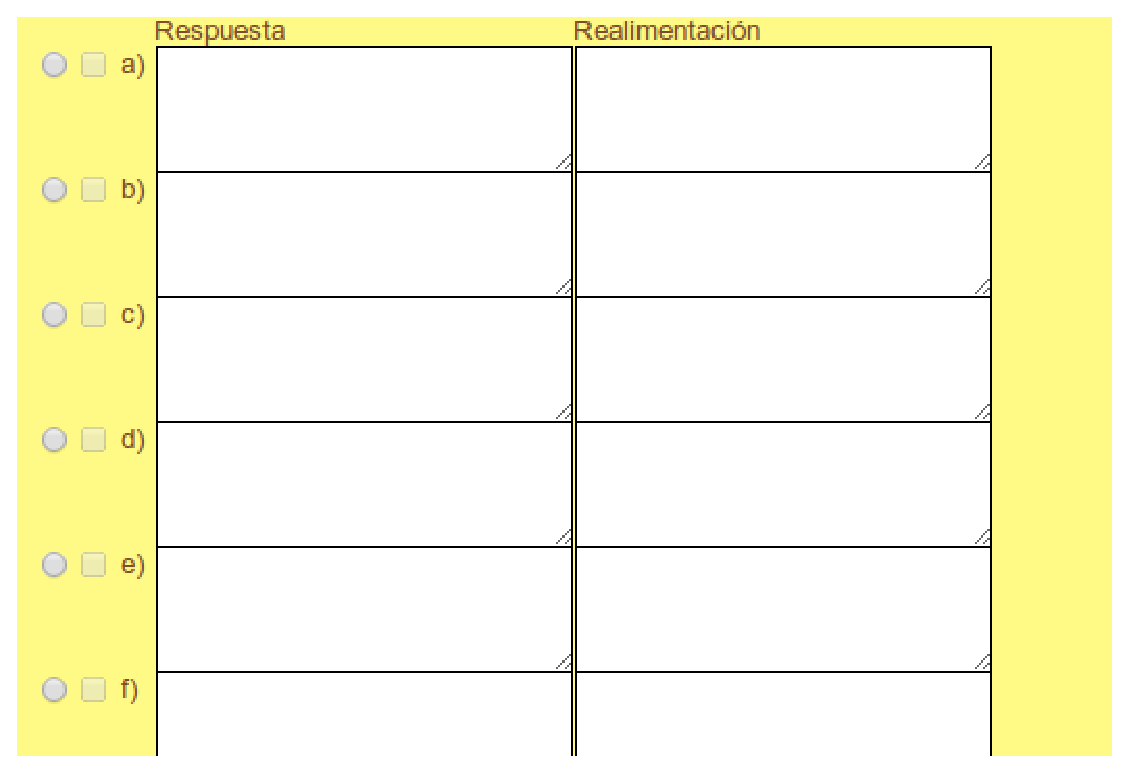
\includegraphics[width=4in]{fig/inte_test2}
  \caption{Creación de un nuevo test. Respuestas.}
  \label{fig:inte_test2}

\end{figure}


Finalmente debemos instanciar SWADE en los mensajes de SWAD, ya sea Mensajes entre usuarios o en los Foros. En principio no será necesario integrarlo en los Avisos. Tampoco es necesario en principio integrarlo en Convocatoria de examen o los Campos de las fichas. En la figura ~\ref{fig:inte_men} podemos ver donde tendremos que insertar el editor para los mensajes.

\begin{figure}[h!]
  \centering
      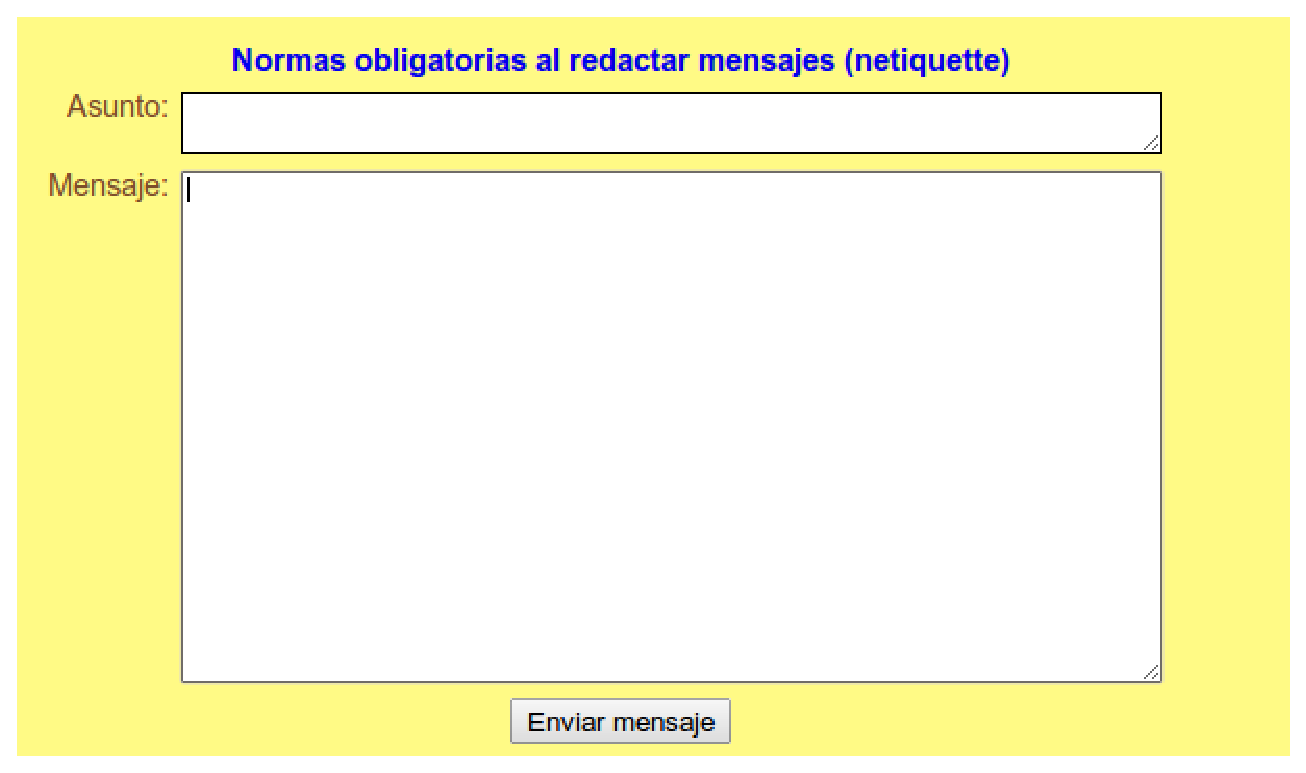
\includegraphics[width=4in]{fig/inte_men}
  \caption{Mensajes de SWAD}
  \label{fig:inte_men}

\end{figure}
